\documentclass[12pt]{article}

\setlength{\parindent}{0pt}
\setcounter{secnumdepth}{3}
\usepackage[margin=1in]{geometry}

% packages
\usepackage{amsmath, amsfonts, amsthm, amssymb}
\usepackage{graphicx, float}
\usepackage{mathtools}
\usepackage{titlesec}
\usepackage{interval}
\usepackage{hyperref}
\usepackage{siunitx}
\usepackage{titling}
\usepackage{vwcol}
\usepackage{setspace}
\usepackage{empheq}
\usepackage{cancel}
\usepackage{esdiff}
\usepackage{multicol}
\usepackage{mdframed}
\usepackage{esdiff}
\usepackage{tikzsymbols}
\usepackage{multicol}
\usepackage{tikz}
\usepackage{varwidth}
\usepackage{pgfplots}
\usepackage{fancyhdr}
\usepackage{enumitem}
\usepackage{tcolorbox}

\intervalconfig {
	soft open fences
}

% header
\pagestyle{fancy}
\fancyhf{}
\lhead{Ethan Fan}
\rhead{PCH}
\cfoot{\thepage}

% section format
\titleformat{\section}
  {\bfseries}
  {}
  {0em}
  {}
\titlespacing*{\section}{0pt}{0pt}{0.3em}

\titleformat{\subsection}[runin]
  {\bfseries}
  {}
  {0em}
  {}
\titlespacing*{\subsection}{0pt}{0pt}{0em}

\titleformat{\subsubsection}[runin]
  {\itshape}
  {(\roman{subsubsection})}
  {0em}
  {}

% commands
\newcommand{\alignedintertext}[1]{%
  \noalign{%
    \vskip\belowdisplayshortskip
    \vtop{\hsize=\linewidth#1\par
    \expandafter}%
    \expandafter\prevdepth\the\prevdepth
  }%
}

\newcommand*{\paren}[1]{\ensuremath\left(#1\right)}
\newcommand*{\limit}[2][x]{\ensuremath{\displaystyle\lim_{#1\to#2}}}
\newcommand*{\Limit}[3][x]{\ensuremath{\displaystyle\lim_{#1\to#2}\left[#3\right]}}
\newcommand*{\deriv}[1][x]{\ensuremath{\dfrac{\mathrm{d}}{\mathrm{d}#1}}}
\newcommand*{\Deriv}[2][x]{\ensuremath{\dfrac{\mathrm{d}}{\mathrm{d}#1}\left[#2\right]}}
\newcommand{\dydx}{\frac{dy}{dx}}
\newcommand*{\iinteg}[2][x]{\ensuremath{\displaystyle\int #2\;\mathrm{d}#1}}
\newcommand*{\dinteg}[4][x]{\ensuremath{\displaystyle\int_{#2}^{#3}#4\;\mathrm{d}#1}}
\newcommand*{\abs}[1]{\ensuremath{\left|#1\right|}}
\newcommand*{\eps}{\varepsilon}
\newcommand*{\real}{\ensuremath\mathbb{R}}
\newcommand*{\integer}{\ensuremath\mathbb{Z}}
\newcommand*{\posint}{\ensuremath\mathbb{Z^+}}
\newcommand*{\cbrt}[1]{\ensuremath{\sqrt[3]{#1}}}
\newcommand*{\lheqzero}{\ensuremath{\underset{\text{L'H}}{\overset{\left[\frac00\right]}{=}}}}
\newcommand*{\lheqinfty}{\ensuremath{\underset{\text{L'H}}{\overset{\left[\frac{\infty}{\infty}\right]}{=}}}}
\newcommand{\tor}{\text{ or }}
\newcommand{\floor}[1]{\lfloor #1 \rfloor}

\newcommand{\vem}{\vspace{0.5em}}
\newcommand{\example}[1]{\section{Example #1}}
\newcommand{\problem}[1]{\section{Problem #1}}
\newcommand{\subproblem}[1]{\subsection{(#1)} \,}

\DeclareMathOperator{\dne}{DNE}
\DeclareMathOperator{\sgn}{sgn}

\newcommand{\definition}[1]{\begin{tcolorbox}[colback=red!5!white,colframe=red!75!black,parbox=false] #1 \end{tcolorbox}}

\newcommand{\theorem}[2]{\begin{tcolorbox}[title={#1},colback=blue!5!white,colframe=blue!75!black,parbox=false] #2 \end{tcolorbox}}

\allowdisplaybreaks
% \postdisplaypenalty=100000

% document
\begin{document}

\vspace*{0cm}

% opening
\begin{center}
    {\Large \bfseries Problem Set 73} \\[0.5cm]
    {\large Indeterminate Forms and L'Hopital's Rule} \\[0.35cm]
    {\normalsize May 7, 2026}
\end{center}

% problems

\problem{2}
Find the limit: \vem

\subproblem{a} $\lim\limits_{x \to 0^+} x^{x^2}$
\begin{gather*}
    \lim\limits_{x \to 0^+} x^{x^2} \quad [0^0]\\
    \lim_{x \to 0^+}y=\lim_{x \to 0^+}x^{x^2}\\
    \lim_{x \to 0^+}\ln y =\lim_{x \to 0^+}x^2 \ln x=\lim_{x \to 0^+}\frac{\ln x}{\frac{1}{x^2}}\\
    \begin{cases}
        \lim\limits_{x \to 0^+} \ln x \to -\infty\\
        \lim\limits_{x \to 0^+} \dfrac{1}{x^2} \to \infty
    \end{cases}\\
    \lim_{x \to 0^+}\frac{\ln x}{\frac{1}{x^2}} \underset{\text{L'H}}{\overset{\left[\frac{-\infty}{\infty}\right]}{=}}\lim_{x \to 0^+}\frac{\frac{1}{x}}{-\frac{2}{x^3}}=\lim_{x \to 0^+}-\frac{x^2}{2}=0\\
    \lim_{x \to 0^+}x^{x^2}=\lim_{x \to 0^+}y=e^{\lim_{x \to 0^+} \ln y}=e^0=\boxed{1}
\end{gather*}

\subproblem{b} $\lim\limits_{x \to 0}(1-2x)^\frac{1}{x}$
\begin{gather*}
    \lim\limits_{x \to 0}(1-2x)^\frac{1}{x}\quad [1^\infty]\\
    \lim_{x \to 0}y=\lim_{x \to 0}(1-2x)^\frac{1}{x}\\
    \lim_{x \to 0} \ln y =\lim_{x \to 0} \frac{\ln (1-2x)}{x}\\
    \begin{cases}
        \lim\limits_{x \to 0} \ln (1-2x)=0\\
        \lim\limits_{x \to 0}x=0
    \end{cases}\\
    \lim\limits_{x \to 0}\frac{\ln (1-2x)}{x} \lheqzero \lim\limits_{x \to 0} \frac{-2}{1-2x}=-2\\
    \lim\limits_{x \to 0}(1-2x)^\frac{1}{x}=\lim\limits_{x \to 0}y=e^{\lim\limits_{x \to 0}\ln y}=\boxed{\frac{1}{e^2}}
\end{gather*}

\subproblem{c}
$\lim\limits_{x \to \infty}(1+\dfrac{3}{x}+\dfrac{5}{x^2})^x$
\begin{gather*}
    \lim\limits_{x \to \infty}(1+\dfrac{3}{x}+\dfrac{5}{x^2})^x \quad [1^\infty]\\
    \lim\limits_{x \to \infty}y=\lim\limits_{x \to \infty}(1+\dfrac{3}{x}+\dfrac{5}{x^2})^x\\
    \lim\limits_{x \to \infty} \ln y=\lim\limits_{x \to \infty} x \ln (1+\frac{3}{x}+\frac{5}{x^2})=\lim\limits_{x \to \infty} \frac{\ln (1+\frac{3}{x}+\frac{5}{x^2})}{\frac{1}{x}}\\
    \begin{cases}
        \lim\limits_{x \to \infty} \ln (1+\dfrac{3}{x}+\dfrac{5}{x^2}) =0\\
        \lim\limits_{x \to \infty}\dfrac{1}{x}=0
    \end{cases}\\
    \lim\limits_{x \to \infty} \frac{\ln (1+\frac{3}{x}+\frac{5}{x^2})}{\frac{1}{x}} \lheqzero \lim\limits_{x \to \infty}\dfrac{\dfrac{-\frac{3}{x^2}-\frac{10}{x^3}}{1+\frac{3}{x}+\frac{5}{x^2}}}{-\frac{1}{x^2}}=\lim\limits_{x \to \infty}\frac{3-\frac{10}{x}}{1+\frac{3}{x}+\frac{5}{x^2}}=3\\
    \lim\limits_{x \to \infty}(1+\dfrac{3}{x}+\dfrac{5}{x^2})^x=\lim\limits_{x \to \infty} y =e^{\lim\limits_{x \to \infty} \ln y}=\boxed{e^3}
\end{gather*}

\subproblem{d}
$\lim\limits_{x \to \infty} x^\frac{1}{x}$
\begin{gather*}
    \lim\limits_{x \to \infty} x^\frac{1}{x} \quad [\infty^0]\\
    \lim\limits_{x \to \infty}y=\lim\limits_{x \to \infty} x^\frac{1}{x}\\
    \lim\limits_{x \to \infty} \ln y =\lim\limits_{x \to \infty} \frac{\ln x}{x}\\
    \begin{cases}
        \lim\limits_{x \to \infty} \ln x \to \infty\\
        \lim\limits_{x \to \infty} x \to \infty
    \end{cases}\\
    \lim\limits_{x \to \infty} \frac{\ln x}{x}\lheqzero \lim\limits_{x \to \infty} \frac{1}{x} = 0\\
    \lim\limits_{x \to \infty} x^\frac{1}{x}=\lim\limits_{x \to \infty}y = e^{\lim\limits_{x \to \infty} \ln y} =e^0 =\boxed{1}
\end{gather*}

\subproblem{f}
$\lim\limits_{x\to 0^+}(\cos x)^\frac{1}{x^2}$
\begin{gather*}
    \lim\limits_{x\to 0^+}(\cos x)^\frac{1}{x^2}\quad [1^\infty]\\
    \lim\limits_{x\to 0^+}y=\lim\limits_{x\to 0^+}(\cos x)^\frac{1}{x^2}\\
    \lim\limits_{x\to 0^+}\ln y=\lim\limits_{x\to 0^+}\frac{\ln \cos x}{x^2}\\
    \begin{cases}
        \lim\limits_{x\to 0^+} \ln \cos x=0\\
        \lim\limits_{x\to 0^+}x^2=0
    \end{cases}\\
    \lim\limits_{x\to 0^+} \frac{\ln \cos x}{x^2} \lheqzero \lim\limits_{x\to 0^+} \frac{-\tan x}{2x}\\
    \begin{cases}
        \lim\limits_{x\to 0^+} -\tan x=0\\
        \lim\limits_{x\to 0^+} 2x =0
    \end{cases}\\
    \lim\limits_{x\to 0^+} \frac{-\tan x}{2x} \lheqzero \lim\limits_{x\to 0^+} \frac{-\sec^2 x}{2}=-\frac{1}{2}\\
    \lim\limits_{x\to 0^+} (\cos x)^\frac{1}{x^2}=\lim\limits_{x\to 0^+}y = e^{\lim\limits_{x\to 0^+} \ln y}= \boxed{\frac{1}{\sqrt{e}}}
\end{gather*}

\problem{3}
Let $f(x)=e^x-1$, $g(x)=x^3+4x$. \vem

\subproblem{a}
Illustrate L'Hopital's Rule by graphing both $\dfrac{f(x)}{g(x)}$ and $\dfrac{f'(x)}{g'(x)}$ near $x=0$ to see that these ratios have the same limit as $x\to 0$.
\begin{figure}[H]
    \centering
    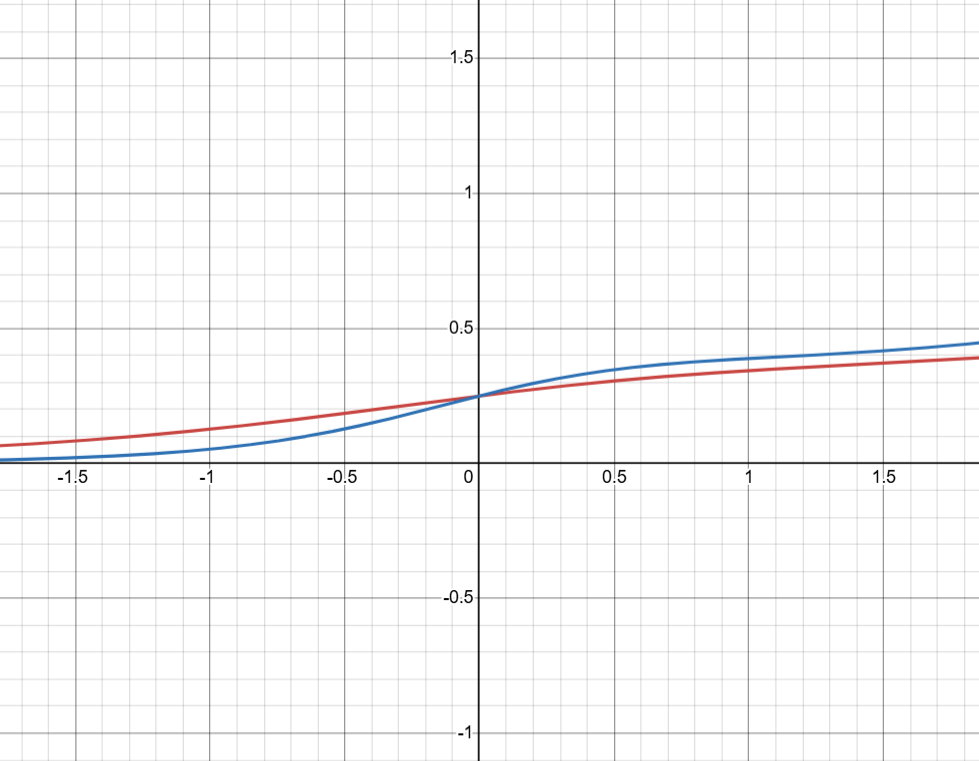
\includegraphics[width=0.5\linewidth]{q3.png}
\end{figure}

\subproblem{b}
Calculate the exact value of the limit.
\begin{gather*}
    \lim\limits_{x \to 0} \frac{e^x-1}{x^3+4x}\quad \left[\frac{0}{0}\right]\\
    \begin{cases}
        \lim\limits_{x \to 0} e^x-1=0\\
        \lim\limits_{x \to 0} x^3+4x=0
    \end{cases}\\
    \lim\limits_{x \to 0}\frac{e^x-1}{x^3+4x}\lheqzero \lim\limits_{x \to 0} \frac{e^x}{3x^2+4}=\boxed{\frac{1}{4}}
\end{gather*}

\problem{7}
If an initial amount of money $A_0$ is invested at an interest rate $r$ compounded $n$ times a year, the value of the investment after $t$ years is
$$A = A_0 \left( 1 + \frac{r}{n} \right)^{nt}.$$
If we let $n \to \infty$, we refer to the continuous compounding of interest. Use L'Hôpital's Rule to show that if interest is compounded continuously, then the amount after $t$ years is
$$A = A_0 e^{rt}.$$
\begin{gather*}
    \lim\limits_{n \to \infty}y=\lim\limits_{n \to \infty}(1+\frac{r}{n})^{nt}\quad [1^\infty]\\
    \lim\limits_{n \to \infty}\ln y=\lim\limits_{n \to \infty} nt \ln (1+\frac{r}{n})=\lim\limits_{n \to \infty}\frac{\ln (1+\frac{r}{n})}{\frac{1}{nt}}\\
    \begin{cases}
        \lim\limits_{n \to \infty} \ln (1+\dfrac{r}{n})=0\\
        \lim\limits_{n \to \infty}\dfrac{1}{nt}=0
    \end{cases}\\
    \lim\limits_{n \to \infty}\frac{\ln (1+\frac{r}{n})}{\frac{1}{nt}} \lheqzero \lim\limits_{n \to \infty}\frac{\frac{-\frac{r}{n^2}}{1+\frac{r}{n}}}{-\frac{1}{n^2t}}= \lim\limits_{n \to \infty} \frac{rt}{1+\frac{r}{n}}=rt\\
    \lim\limits_{n \to \infty} y = e^{\lim\limits_{n \to \infty} \ln y} = e^{rt}\\
    A=A_0 \lim\limits_{n \to \infty}(1+\frac{r}{n})^{nt} =\boxed{A_0e^{rt}}
\end{gather*}

\problem{8}
If $f'$ is continuous, $f(2) = 0$, and $f'(2) = 7$, evaluate
$$\lim_{x \to 0} \frac{f(2 + 3x) + f(2 + 5x)}{x}.$$
\begin{align*}
    \lim_{x \to 0} \frac{f(2 + 3x) + f(2 + 5x)}{x}&= \lim_{x \to 0}\frac{f(2+3x)}{x}+\lim_{x \to 0}\frac{f(2+5x)}{x}\\
    &=3\lim_{x \to 0}\frac{f(2+3x)-f(2)}{3x} +5\lim_{x \to 0}\frac{f(2+5x)-f(2)}{5x}\\
    &=3f'(2)+5f'(2)\\
    &=\boxed{56}
\end{align*}

\problem{9}
Prove that
$$\lim_{x \to \infty} \frac{\ln x}{x^p} = 0$$
for any number $p > 0$. This shows that the logarithmic function approaches $\infty$ more slowly than any power of $x$
\begin{gather*}
    \begin{cases}
        \lim\limits_{x \to \infty} \ln x \to \infty\\
        \lim\limits_{x \to \infty} x^p \to \infty
    \end{cases}\\
    \lim\limits_{x \to \infty} \frac{\ln x}{x^p}\lheqinfty \lim\limits_{x \to \infty} \frac{x^{-1}}{px^{p-1}}=\lim\limits_{x \to \infty}\frac{1}{px^p}=\boxed{0}
\end{gather*}

\problem{10}
Prove that
$$\lim_{x \to 0^+} x^\alpha \ln x = 0$$
for any $\alpha > 0$.
\begin{gather*}
    \lim\limits_{x \to 0^+} x^\alpha \ln x =  \lim\limits_{x \to 0^+} \frac{\ln x}{\frac{1}{x^{\alpha}}}\\
    \begin{cases}
        \lim\limits_{x \to 0^+} \ln x \to -\infty\\
        \lim\limits_{x \to 0^+} \dfrac{1}{x^a} \to \infty
    \end{cases}\\
    \lim\limits_{x \to 0^+}\frac{\ln x}{\frac{1}{x^\alpha}}\underset{\text{L'H}}{\overset{\left[\frac{-\infty}{\infty}\right]}{=}} \lim\limits_{x \to 0^+} \frac{x^{-1}}{-\alpha x^{-\alpha -1}}=\lim\limits_{x \to 0^+}-\frac{x^{\alpha}}{\alpha }=\boxed{0}
\end{gather*}


\end{document}

